
\documentclass[12pt, a4paper]{article} %Dokumentinformationen/Präambel
\usepackage{graphicx} %Paket für Bilder
\usepackage{caption} %Paket für Bildunterschriften
\usepackage[german]{babel} %Paket für Rechtschreibung
\usepackage{listings}
\usepackage{titlesec}
\usepackage{tikz}
\usepackage{float}
\usetikzlibrary{tikzmark}
\usetikzlibrary{matrix}
\usepackage{array}
\UseRawInputEncoding
\usepackage{color}
% Für Quelltext
\usepackage{listings}
\usepackage{color}
\definecolor{mygreen}{rgb}{0,0.6,0}
\definecolor{mygray}{rgb}{0.5,0.5,0.5}
\definecolor{mymauve}{rgb}{0.58,0,0.82}
\lstset{
  keywordstyle=\color{blue},commentstyle=\color{mygreen},
  stringstyle=\color{mymauve},rulecolor=\color{black},
  basicstyle=\footnotesize\ttfamily,numberstyle=\tiny\color{mygray},
  captionpos=b, % sets the caption-position to bottom
  keepspaces=true, % keeps spaces in text
  numbers=left, numbersep=5pt, showspaces=false,showstringspaces=true,
  showtabs=false, stepnumber=2, tabsize=2, title=\lstname}

\begin{document} %Beginn des eigentlichen Dokuments

\thispagestyle{empty}

%Beginn Titelseite
\begin{title}
	
	\centering{\scshape\Large Projektwoche 2022 am EMA \par}
	\vspace{5cm}
	
	{\scshape\Huge Mein erstes LaTex Dokument \par}

	\vspace{5cm}
	{\Large\itshape Tim \par} %Hier deinen Namen eintragen
	

\end{title}
%Ende Titelseite

\newpage

\tableofcontents %erzeugt Inhaltsverzeichnis automatisch

\newpage

\section{\"Uber mich}

%Hier folgt eine Möglichkeit, etwas in LaTex aufzulisten
\begin{description}
\item[Name.]
Tim %Hier eintragen
\item[Alter.] 
12 
\item[Hobbys.]
Skaten
\item[Lieblingsfach.]
ich hasse Schule
\item[Lieblingsessen.]
Glutenfreie Pizza
\item[Lieblingsmusik.]
Oldschool Hiphop, Rap 
\item[Lieblingsmusiker] %Eigenen Punkt erstellen
Eazy E Ice Cube
\end{description}

\section{Bild in LaTex}
\begin{figure} 
%Lade im Internet ein Bild herunter, lade es in Overleaf hoch und binde es mit dem Befehl

\includegraphics[height=100mm]{Kevin.jpeg}
\caption{Kevin und sein Gesicht}

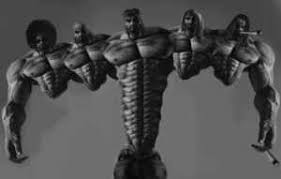
\includegraphics[height=100mm]{Gigachad.jpeg}
\end{figure}
%	\includegraphics[height=50mm]{Dateiname}
%in LaTex ein
%Mit dem Befehl
%	\caption{Bildunterschrift}
%kannst du eine Bildunterschrift hinzufügen, z.B. die Quelle
\begin{figure}[h]%h = here (t = top; b = bottom; p = page)
\centering %Hier Befehl eingeben
\end{figure}

\section{Arten von Kapiteln}
\subsection{Unterkapitel}
Mit \verb|\section{Name}| beginnst du ein neues Kapitel, was automatisch im Inhaltsverzeichnis angezeigt wird, sofern der Befehl \verb|\tableofcontents| auf der entsprechenden Seite eingebunden ist.
\subsubsection{UnterUnterUnterKapitel}
\subsection{Unterkapitel}

Mit \verb|\subsection{Name}| f\"ugst du ein Unterkapitel ein.

\subsubsection{Unterunterkapitel}

Mit \verb|\subsubsection{Name}| f\"ugst du ein Unterunterkapitel ein.

\section{Textgr\"o\ss e}

%Im Dokumentkopf (Zeile 1) legst du die Default-Schriftgröße des Dokuments fest (hier sind das 12pt). Wenn du z.B. auf der Titelseite andere Schriftgrößen verwenden möchtest, 
%helfen folgende Befehle.

%Du änderst die Schriftgröße mit
%	\Schriftgröße
% Die Namen dieser Größen stehen in der Tabelle

%Ersetze die 'x' in der Tabelle mit einem Wort in der entsprechenden Schriftart, welche links daneben steht


\begin{table}[h] 
\centering
\begin{tabular}{l | l}
\bf{Gr\"o\ss e} & \bf{Beispiel} \\
\hline 
Huge & x\\
\hline
huge & x\\
\hline
LARGE & x\\
\hline
Large & x\\
\hline 
large & x\\
\hline
normalsize & x\\
\hline
small & x\\
\hline
footnotesize & x\\
\hline
scriptsize & x\\
\hline
tiny & x\\
\end{tabular}
\caption{\label{tab4}Schriftgr\"o\ss en in LaTex }
\end{table}

\section{Textfarbe}

%Erkundige dich im Internet, wie man Farben in LaTex ändern kann.
%Markiere im folgenden Text beliebige Textpassagen rot, grün, cyan und gelb.

\textcolor{green}{dolor sit amet, consectetur adipiscing elit}, sed do eiusmod tempor incididunt ut labore et dolore magna aliqua. Ut enim ad minim veniam, quis nostrud exercitation ullamco laboris nisi ut aliquip ex ea commodo consequat. Duis aute irure dolor in reprehenderit in voluptate velitesse cillum dolore eu fugiat nulla pariatur
\section{Schriftart}

%Informiere dich auf der Webseite
%	https://de.overleaf.com/learn/latex/Font_sizes%2C_families%2C_and_styles#Font_families
%wie man in LaTex die Schriftart ändern kann

%Schreibe anschließend Passagen im folgenden Text mit folgenden Schriftarten: Roman (upright) serif , sans serif, typewriter (monospace)
\textit{Lorem ipsum dolor sit amet, consectetur adipiscing elit, sed do eiusmod tempor incididunt ut labore et dolore magna aliqua. Ut enim ad minim veniam, quis nostrud exercitation ullamco laboris nisi ut aliquip ex ea commodo consequat. Duis aute irure dolor in reprehenderit in voluptate velit esse cillum dolore eu fugiat nulla pariatur.}
Lorem ipsum dolor sit amet, consectetur adipiscing elit, sed do eiusmod tempor incididunt ut labore et dolore magna aliqua. Ut enim ad minim veniam, quis nostrud exercitation ullamco laboris nisi ut aliquip ex ea commodo consequat. Duis aute irure dolor in reprehenderit in voluptate velit esse cillum dolore eu fugiat nulla pariatur.


\section{Quellcode}

%Mit dem Befehl
%	\begin{lstlisting}[language=*Programmiersprache* ,caption=*Code Name*] ... \end{lstlisting}
%fügst du Quellcode in LaTex ein. Wie du siehst, können die Programmiersprache und der Text unter dem Code
%ausgewählt werden

%Füge in diesem Kapitel entweder einen Quellcode deiner Wahl ein, oder kopiere den Quellcode aus dem Java-Programm im GitHub Ordner:

\end{document}
